% -*- TeX:RNW:UK -*-
\documentclass[10pt]{beamer}\usepackage[]{graphicx}\usepackage[]{color}
% maxwidth is the original width if it is less than linewidth
% otherwise use linewidth (to make sure the graphics do not exceed the margin)
\makeatletter
\def\maxwidth{ %
  \ifdim\Gin@nat@width>\linewidth
    \linewidth
  \else
    \Gin@nat@width
  \fi
}
\makeatother

\definecolor{fgcolor}{rgb}{0.345, 0.345, 0.345}
\makeatletter
\@ifundefined{AddToHook}{}{\AddToHook{package/xcolor/after}{\definecolor{fgcolor}{rgb}{0.345, 0.345, 0.345}}}
\makeatother
\newcommand{\hlnum}[1]{\textcolor[rgb]{0.686,0.059,0.569}{#1}}%
\newcommand{\hlstr}[1]{\textcolor[rgb]{0.192,0.494,0.8}{#1}}%
\newcommand{\hlcom}[1]{\textcolor[rgb]{0.678,0.584,0.686}{\textit{#1}}}%
\newcommand{\hlopt}[1]{\textcolor[rgb]{0,0,0}{#1}}%
\newcommand{\hlstd}[1]{\textcolor[rgb]{0.345,0.345,0.345}{#1}}%
\newcommand{\hlkwa}[1]{\textcolor[rgb]{0.161,0.373,0.58}{\textbf{#1}}}%
\newcommand{\hlkwb}[1]{\textcolor[rgb]{0.69,0.353,0.396}{#1}}%
\newcommand{\hlkwc}[1]{\textcolor[rgb]{0.333,0.667,0.333}{#1}}%
\newcommand{\hlkwd}[1]{\textcolor[rgb]{0.737,0.353,0.396}{\textbf{#1}}}%
\let\hlipl\hlkwb

\usepackage{framed}
\makeatletter
\newenvironment{kframe}{%
 \def\at@end@of@kframe{}%
 \ifinner\ifhmode%
  \def\at@end@of@kframe{\end{minipage}}%
  \begin{minipage}{\columnwidth}%
 \fi\fi%
 \def\FrameCommand##1{\hskip\@totalleftmargin \hskip-\fboxsep
 \colorbox{shadecolor}{##1}\hskip-\fboxsep
     % There is no \\@totalrightmargin, so:
     \hskip-\linewidth \hskip-\@totalleftmargin \hskip\columnwidth}%
 \MakeFramed {\advance\hsize-\width
   \@totalleftmargin\z@ \linewidth\hsize
   \@setminipage}}%
 {\par\unskip\endMakeFramed%
 \at@end@of@kframe}
\makeatother

\definecolor{shadecolor}{rgb}{.97, .97, .97}
\definecolor{messagecolor}{rgb}{0, 0, 0}
\definecolor{warningcolor}{rgb}{1, 0, 1}
\definecolor{errorcolor}{rgb}{1, 0, 0}
\makeatletter
\@ifundefined{AddToHook}{}{\AddToHook{package/xcolor/after}{
\definecolor{shadecolor}{rgb}{.97, .97, .97}
\definecolor{messagecolor}{rgb}{0, 0, 0}
\definecolor{warningcolor}{rgb}{1, 0, 1}
\definecolor{errorcolor}{rgb}{1, 0, 0}
}}
\makeatother
\newenvironment{knitrout}{}{} % an empty environment to be redefined in TeX

\usepackage{alltt}
\usetheme{metropolis}
%\useinnertheme{rectangles}
\setbeamercovered{%
still covered={\opaqueness<1->{15}},
again covered={\opaqueness<1->{40}}}

\hypersetup{colorlinks,linkcolor=black,urlcolor=brown,citecolor=brown}

\usepackage{amsmath,amssymb,amsthm}
\usepackage{unicode-math}

% We set the Lucida OTF fonts as default
\usepackage{fontspec}
\setmainfont{Lucida Bright OT}
\setsansfont{Lucida Sans OT}
\setmonofont{Lucida Console DK}[Scale=MatchLowercase]

\newfontfamily\webglyphsfont{WebHostingHub-Glyphs}[Scale=0.7]
\newcommand\webglyphs[1]{{\webglyphsfont\symbol{#1}}}
\newcommand\Discussion{\colorbox{white}{\textcolor{black}{\webglyphs{"F134}}}\xspace}
\newcommand\DiscussionI{\colorbox{black}{\textcolor{white}{\webglyphs{"F134}}}\xspace}
\newcommand\DExamples{\colorbox{black}{\textcolor{white}{\webglyphs{"F134} examples?}}}
\newcommand\Reading{\colorbox{black}{\textcolor{white}{\webglyphs{"F0C1}}}\xspace}
\newcommand\ReadingI{\colorbox{white}{\textcolor{black}{\webglyphs{"F0C1}}}\xspace}
\newcommand\Video{\colorbox{white}{\textcolor{black}{\webglyphs{"F03D}}}\xspace}
\newcommand\Attention{\colorbox{black}{\textcolor{orange}{\webglyphs{"F05A}}}\xspace}
\newcommand\HomeWork{\colorbox{white}{\textcolor{black}{\webglyphs{"F5ED}}}\xspace}
\newcommand\HomeWorkI{\colorbox{black}{\textcolor{white}{\webglyphs{"F5ED}}}\xspace}
\newcommand\Advanced{\colorbox{black}{\textcolor{white}{\webglyphs{"F235}}}\xspace}

\newfontfamily\lineabasicfont{linea-basic-10}
\newcommand\basicicons[1]{{\lineabasicfont\symbol{#1}}}
\newcommand\timeforwards{\basicicons{"0079}}
\newcommand\timebackwards{\basicicons{"0064}}

\newfontfamily\lineaweatherfont{linea-weather-10}
\newcommand\weathericons[1]{{\lineaweatherfont\symbol{#1}}}
\newcommand\meteosun{\weathericons{"E038}}
\newcommand\meteosuncloud{\weathericons{"E042}}
\newcommand\meteorain{\weathericons{"E033}}
\newcommand\meteowind{\weathericons{"E054}}

\newfontfamily\uleaffont{Mini Pics Uprooted Leaf}
\newcommand\uleafmpics[1]{{\uleaffont\symbol{#1}}}
\newcommand\lowplants{\uleafmpics{"00CE}}
\newcommand\mediumplant{\uleafmpics{"006A}}
\newcommand\bush{\uleafmpics{"0039}}
\newcommand\smallplant{\uleafmpics{"0030}}
\newcommand\seedling{\uleafmpics{"002F}}
\newcommand\floweringplant{\uleafmpics{"00CA}}

\newfontfamily\utwigfont{Mini Pics Uprooted Twig}
\newcommand\utwigmpics[1]{{\utwigfont\symbol{#1}}}
\newcommand\grassplant{\utwigmpics{"0033}}

\newfontfamily\uinsectfont{Insect Icons}
\newcommand\uinsect[1]{{\uinsectfont\symbol{#1}}}
\newcommand\bug{\uinsect{"006F}}

\usepackage{polyglossia}
\setdefaultlanguage[variant = british, ordinalmonthday = false]{english}

\usepackage[style=authoryear-comp,firstinits,sortcites,maxcitenames=2,%
    mincitenames=1,maxbibnames=10,minbibnames=10,uniquename=mininit,%
    uniquelist=minyear,sortfirstinits=true]{biblatex}
\addbibresource{../references/ecophys.bib}
\renewcommand{\bibfont}{\small}

\usepackage{abbrev}



\usepackage{tikz}
\usetikzlibrary{positioning,fit,arrows}

\tikzset{
 big dot/.style
  = {circle, draw, inner sep=0pt, minimum size=3mm, fill=teal!50},
 a/.style
  = {node distance=4em, text width=0.1em, minimum height=4em},
 b/.style
  = {rectangle, draw, fill=gray!10, node distance=4em, text width=6em,
     text centered, rounded corners, minimum height=4em, thick},
 c/.style
  = {circle, draw, dashed, fill=orange!10, inner sep = 0pt, node distance=5em, text width=6em,
     text centered, thick},
 d/.style
  = {rectangle, draw, dashed, fill=red!10, node distance=4em, text width=6em,
     text centered, rounded corners, minimum height=4em, thick},
 l/.style
  = {draw, -latex, ultra thick},
 lr/.style
  = {draw, latex-latex, ultra thick, red},
 lb/.style
  = {draw, -latex, ultra thick, blue},
  lo/.style
  = {draw, -latex, ultra thick, orange},
  lg/.style
  = {draw, -latex, ultra thick, teal},
  mylabel/.style
  ={text width=6.5em, text centered},
 aa/.style
  = {node distance=4em, text width=0em, minimum height=0.5ex},
 ll/.style
  = {draw, {open triangle 45} -, thick},
 llb/.style
  = {draw, - triangle 45, thick, blue},
 llg/.style
  = {draw, - open triangle 45, thick, green},
  llt/.style
  = {draw, - open triangle 45, thick, teal},
 llr/.style
  = {draw, - triangle 45, thick, purple},
 llo/.style
  = {draw, - triangle 45, thick, orange}
}

\newcommand*{\Px}{\ensuremath{\mathrm{P}}\xspace}
\newcommand*{\Pxfr}{\ensuremath{\mathrm{P_{fr}}}\xspace}
\newcommand*{\Pxr}{\ensuremath{\mathrm{P_r}}\xspace}
\newcommand*{\Pxtot}{\ensuremath{\mathrm{P_{tot}}}\xspace}

%\newcommand*{\COtwo}{\ensuremath{\textrm{CO}_2}\xspace}

\newcommand*{\nEff}{{\scriptsize 0}\xspace}
\newcommand*{\pEff}{\ensuremath{+}\xspace}
\newcommand*{\mEff}{\ensuremath{-}\xspace}
\newcommand*{\uEff}{?\xspace}

\newcommand*{\myatop}[2]{\genfrac{}{}{0pt}{3}{#1}{#2}}
\IfFileExists{upquote.sty}{\usepackage{upquote}}{}
\begin{document}





\title{PBIO-141\\Sensory and Physiological Ecology\\of  Plants}
\subtitle{7: Light sensing}
\author{Pedro J. Aphalo}
\date{January--February 2022}
\institute[Univ.\ of Helsinki]{M.Sc.\ in Plant Biology, University of Helsinki\\[2ex] \url{http://blogs.helsinki.fi/aphalo/}}


  \begin{frame}
    \maketitle
  \end{frame}

  \begin{frame}[c]
    \begin{center}
      \begin{small}
        \copyright 2006--2022 by Pedro J. Aphalo\\
        University of Helsinki, Finland.\\
        \textcolor{blue}{\url{http://blogs.helsinki.fi/senpep-blog/}}\\[2ex]
      \end{small}

      \begin{footnotesize}
        Sensory and Physiological Ecology of Plants slides by Pedro J. Aphalo are licensed under a Creative Commons Attribution-ShareAlike 4.0 International License.

      
\includegraphics[width=6em]{../figures/copyright/by-sa}\\[2ex]
      \end{footnotesize}
        
        \begin{scriptsize}
        Typeset in Lucida Sans, \textrm{Luicda Bright}, \texttt{Lucida Console} and Lucida Math. Icons from fonts ``WebHostingHub Glyphs'' (under SIL-Open Font License) from \url{https://www.webhostinghub.com/}; ``insect icons'' (free from \url{http://www.woodcutter.es/}); ``linea-basic-10'' and ``linea-weather-10'' (free from \url{https://github.com/linea-io}), ``Mini Pics Uprooted Twig'' and ``Mini Pics Uprooted Twig'' (commercial, from Image Club Graphics, Inc.). Plant icon as .svg by Abdul Wahhab (free from \url{NounProject.com}).

        Illustrations and text quoted from copyrighted sources is excluded from this license and their use should respect the original licenses.
        \end{scriptsize}
    \end{center}
  \end{frame}


  \begin{frame}
    \frametitle{Outline}
    \tableofcontents
  \end{frame}

\section{Responses to shade (cont.)}

\begin{frame}{Timing of shade}{}
    {\footnotesize  \textit{Arabidopsis} seedlings \autocite[from][]{Sellaro2012}.\\}
    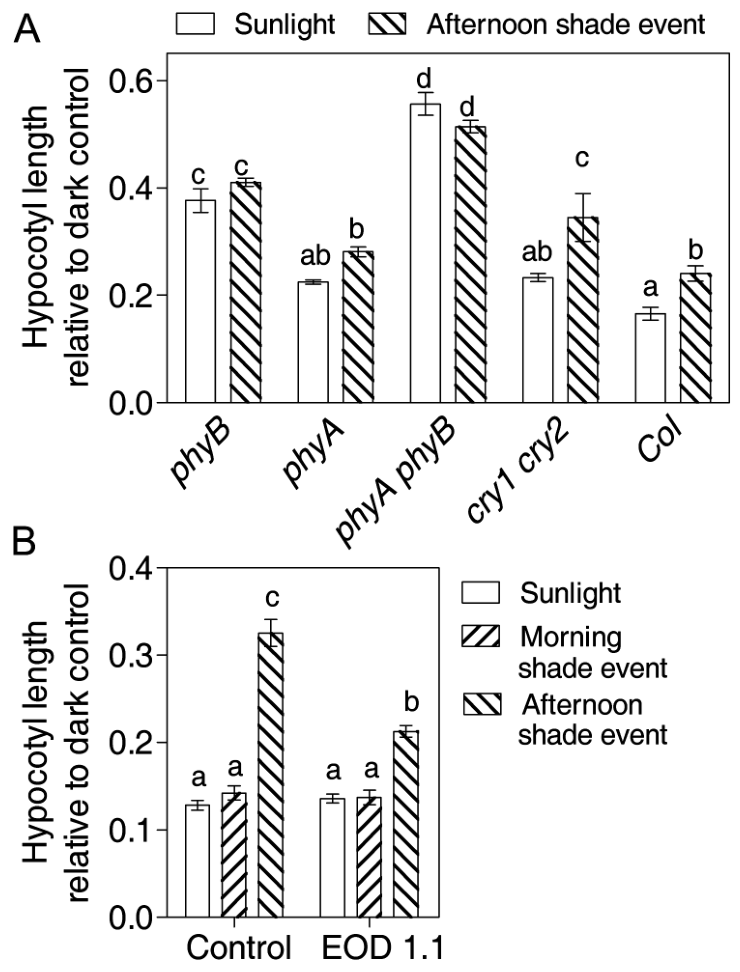
\includegraphics[height=0.85\textheight]{../figures/Sellaro2012-afternoon-shade}
\end{frame}

\begin{frame}{Sunflecks, UVR8, CRY1}{}
    {\footnotesize \textit{Arabidopsis} seedlings \autocite[from][]{Moriconi2018}. In A \mmol should read \umol.\\}
    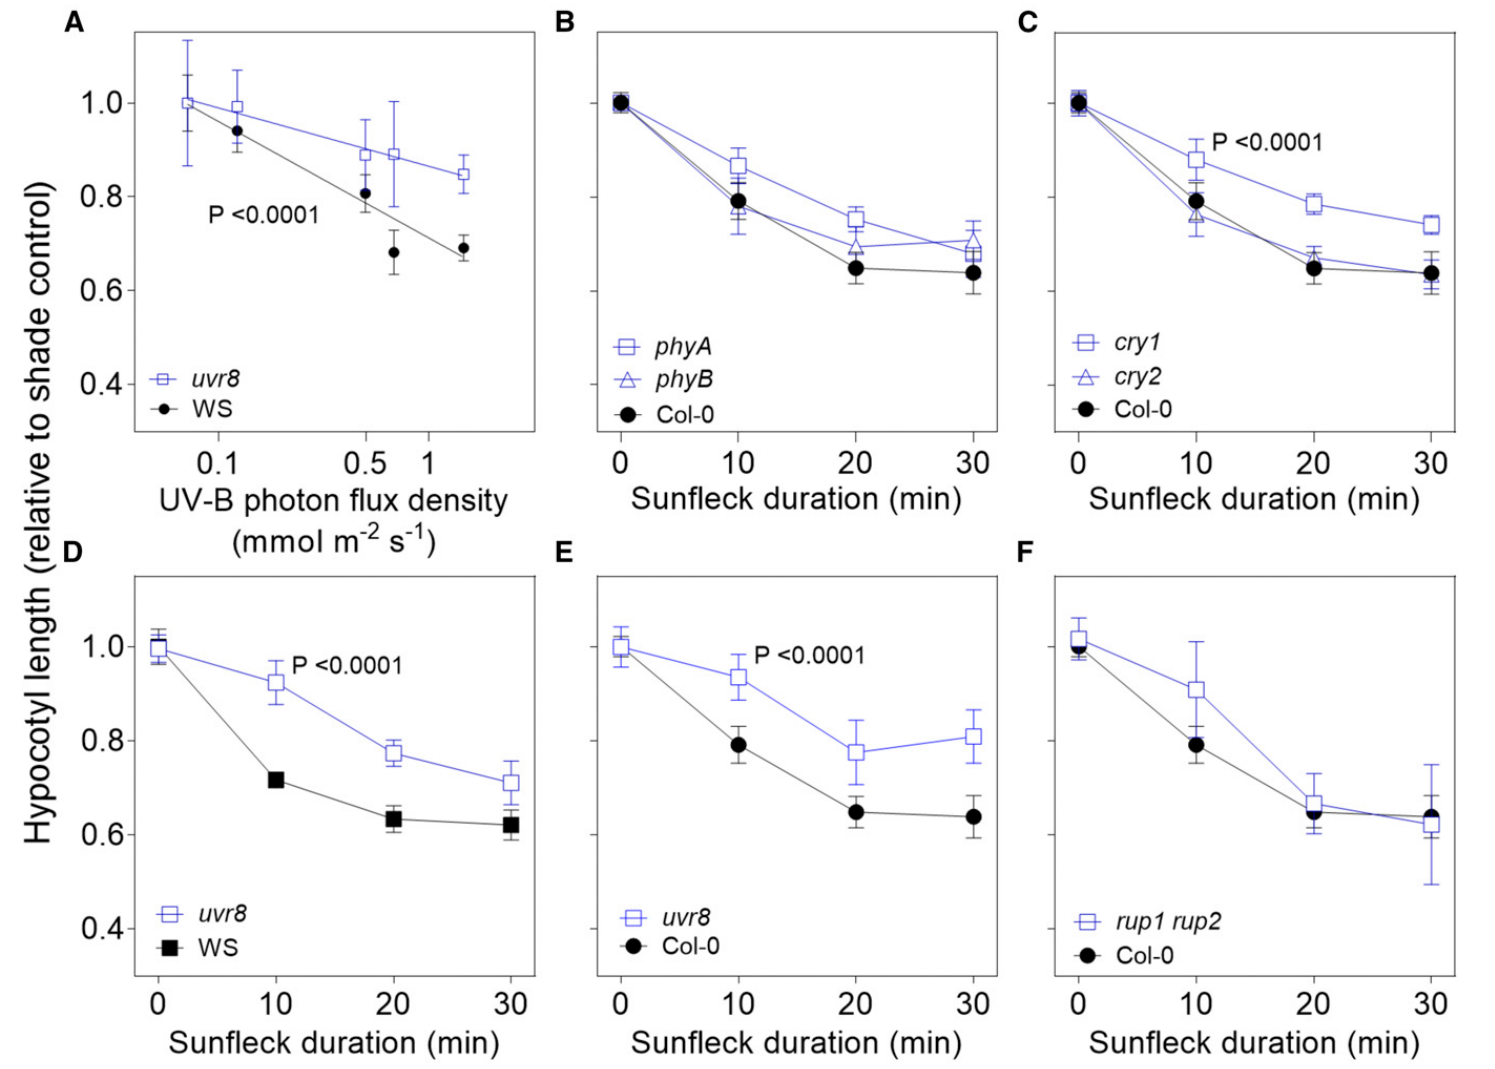
\includegraphics[width=0.9\textwidth]{../figures/Moriconi2018-UVR8-sunflecks}
\end{frame}

\begin{frame}
  \frametitle{Preemptive acclimation: shade}

\footnotesize
\resizebox{\linewidth}{!}{%
  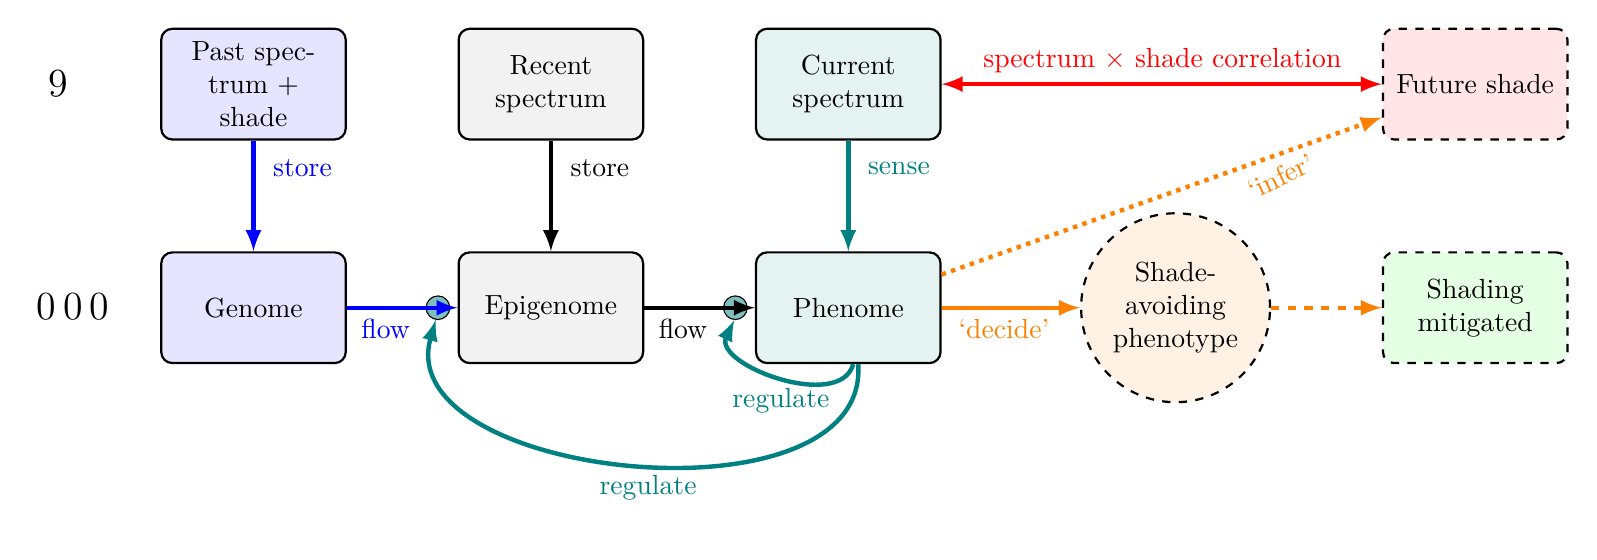
\begin{tikzpicture}[auto]
    \node [a] (environment) {\Large\meteosun\bush};
    \node [b, right = of environment, fill=blue!10] (history) {Past spectrum + shade};
    \node [b, right = of history] (stress) {Recent spectrum};
    \node [b, right = of stress, fill=teal!10] (data) {Current spectrum};
    \node [b, below = of history, fill=blue!10] (genome) {Genome};
    \node [big dot, right = of genome] (valve1) {};
    \node [b, below = of stress] (memory) {Epigenome};
    \node [big dot, right = of memory] (valve2) {};
    \node [b, right = of memory, fill=teal!10] (info) {Phenome};
    \node [a, below = of environment] (plant) {\Large\smallplant\,\smallplant\,\smallplant};
    \node [c, right = of info, fill=orange!10] (acclimation) {Shade-avoiding phenotype};
    \node [d, right = of acclimation, fill=green!10] (ready) {Shading mitigated};
    \node [d, above = of ready] (stress2) {Future shade};

    \path [l] (stress) -- (memory) node[near start,right]{\hspace{0.3em}store};
    \path [lb] (history) -- (genome) node[near start, right]{\hspace{0.3em}store};
    \path [lg] (data) -- (info) node[near start,right]{\hspace{0.3em}sense};
    \path [lb] (genome) -- (memory) node[near start,below]{\hspace{0.8em}flow};
    \path [l] (memory) -- (info) node[near start,below]{\hspace{0.8em}flow};
    \path [lr] (stress2) -- (data) node[near end,above]{\hspace{8em}spectrum $\times$ shade correlation};
    \path [lo, dotted] (info) -- (stress2) node[near end,below,rotate=25]{`infer'};
    \path [lo] (info) -- (acclimation) node[near start,below]{\hspace{2em}`decide'};
    \path [lo, dashed] (acclimation) -- (ready);
    \path [lg] (info) edge [bend left=100]  node[midway, below]{\hspace{1em}regulate} (valve1);
    \path [lg] (info) edge [bend left=95]  node[midway, below]{regulate\hspace{5em}} (valve2);
\end{tikzpicture}%
}%

{\tiny Flow of information in preemptive acclimation to shade by perception of radiation changes. Arrows represent flows of information: \textcolor{blue}{\textbf{blue}} = retrieved from genome (stored during earlier generations), \textbf{black} = acquired and/or `memorized' during an individual's or its progenitor's lifetime, \textcolor{teal}{\textbf{teal}} = regulation of gene expression by phenome or downward causation, \textcolor{red}{\textbf{red}} = lagged correlation between early changes in spectral irradiance and future low PAR irradiance, \textcolor{orange}{\textbf{orange}} = outcome of information processing: a `decision', based on an `implicit forecast of impending shade', leading to developmental adjustments that would increase the probability of higher fitness in the presence of neighbours in comparison with phenotypes lacking preemptive acclimation. \textcolor{green}{\textbf{green}} = `Shading mitigated' compared, in probabilistic terms, to no acclimation. Dashed boxes and arrows represent the likely or forecasted future.}
\end{frame}

\begin{frame}
  \frametitle{Preemptive acclimation: What is the evidence?}
  \begin{itemize}
    \item Several plant responses can be only explained from the evolutive/fitness point of view as being a `preparation' to tolerate or escape future stress events or take advantage of future favourable conditions.
    \item Preemptive shade avoidance as a response to reflected far-red light from neighbouring plants.
    \item Winter hardening and dehardening, timing of bud burst, timing of flowering, etc.
    \item \emph{Anticipatory responses} and \emph{future perception} are terms also used in this context.
  \end{itemize}
\end{frame}

\begin{frame}{Acclimation vs.\ rapid/reversible responses \Discussion 5 min}{}
    {\footnotesize \autocite[from][]{Casal2013a}. What about the balance between light reactions and carbon reactions of photosynthesis?\\}
    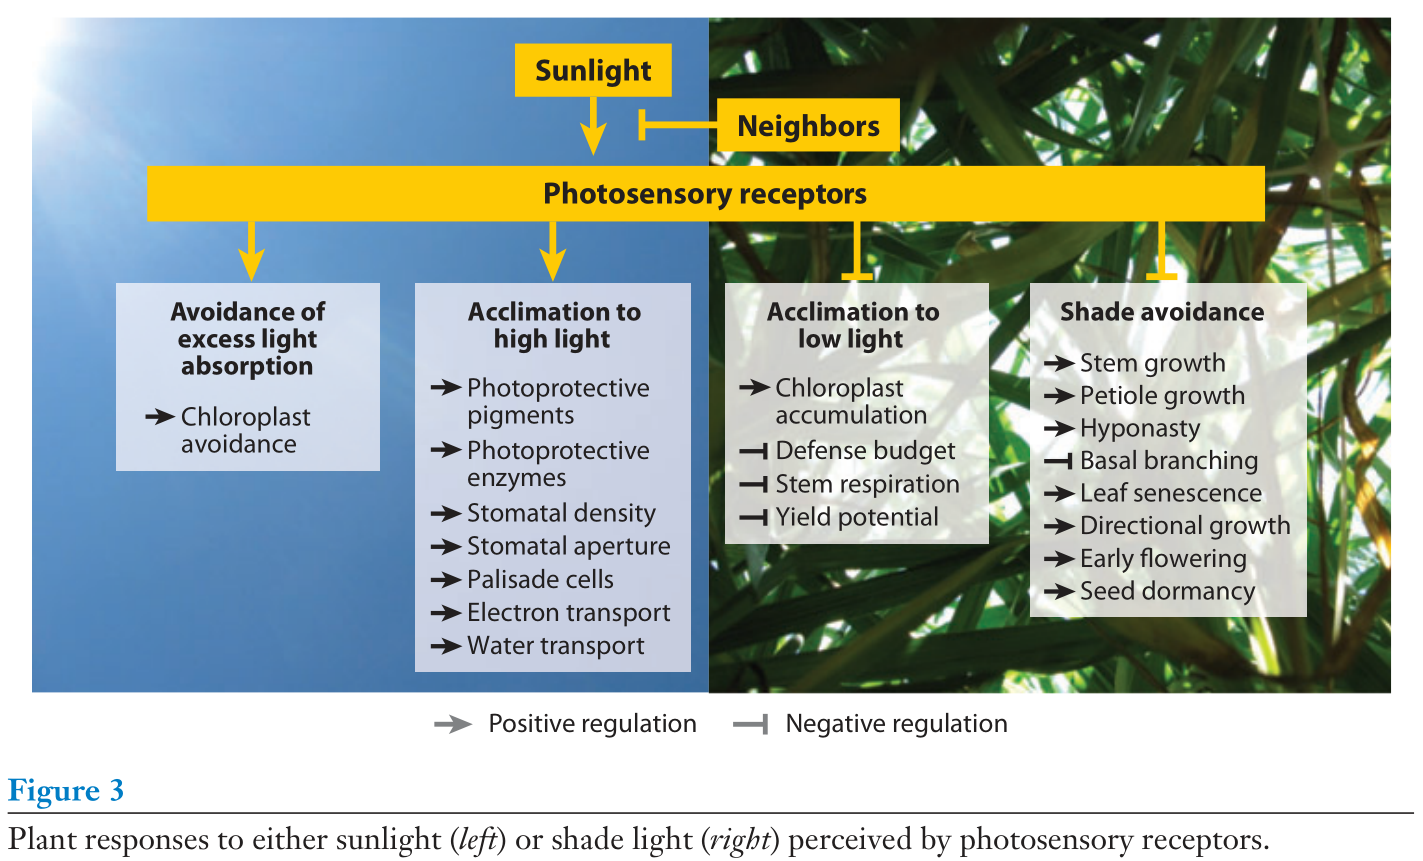
\includegraphics[width=0.98\textwidth]{../figures/Casal2013a-Fig3}
\end{frame}

\section{The photoreceptors}

\begin{frame}{Role of photoreceptors in responses to shade}{}
    {\footnotesize \autocite[from][]{Casal2013a}.\\}
    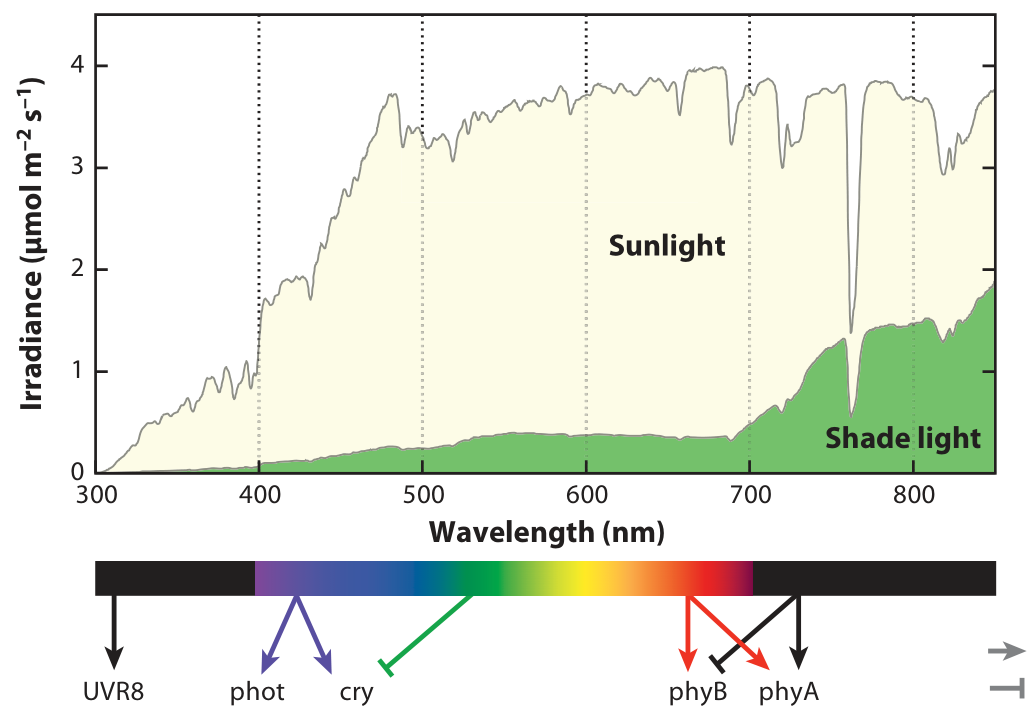
\includegraphics[width=0.98\textwidth]{../figures/Casal2013a-Fig2a}
\end{frame}

\begin{frame}{Photoreceptors: Chromophores}
  \begin{itemize}
    \item Photoreceptors are proteins, like enzymes
    \item Except for UVR8 (UVB photoreceptor) the light is not absorbed by the protein
    \item A different type of molecule coupled to the protein absorbs the photons
    \item The type of chromophore is the main determinant of what wavelengths are absorbed
    \item The protein transfers the energy through different mechanisms to a signalling pathway
    \item In most cases changes in gene expression are triggered
  \end{itemize}
\end{frame}

\begin{frame}{Photoreceptors vs.\ wavelength}{}
    {\footnotesize Several variations on this figure exist \autocite[from][]{Rai2020}.\\}
    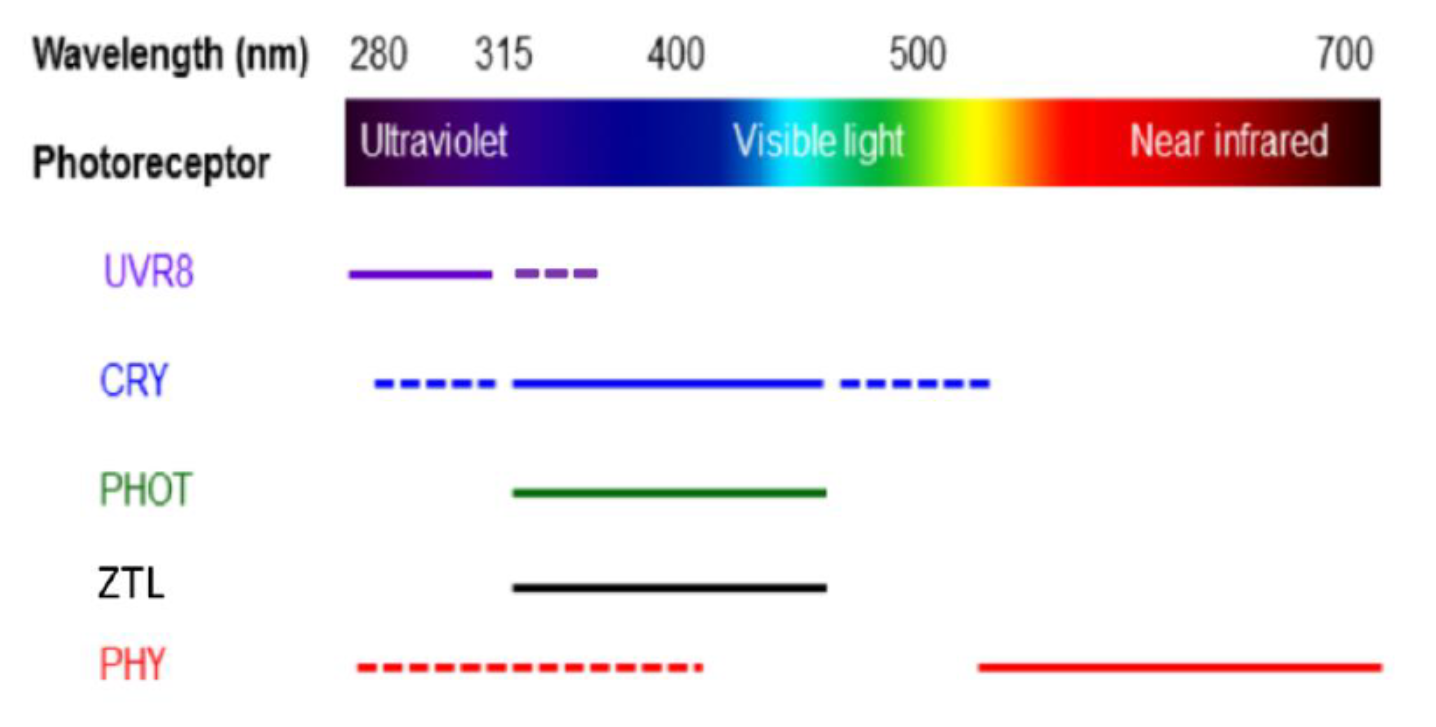
\includegraphics[width=0.98\textwidth]{../figures/photoreceptors-wlength-Rai}
\end{frame}

\begin{frame}{Photoreceptors}
    \begin{itemize}
            \item Phytochromes: PhyA, PhyB, PhyC, PhyD, PhyE
            \item Cryptochromes: Cry1, Cry2, (Cry3)
            \item Phototropins: Phot1, Phot2
            \item UV-receptor: UVR8
            \item Blue-green receptor: (Zeaxanthin)
            \item other LOV-containing proteins
            \item ?
    \end{itemize}
\end{frame}

\begin{frame}{Photoreceptors: Phy (in vitro)}
\begin{knitrout}\tiny
\definecolor{shadecolor}{rgb}{0.969, 0.969, 0.969}\color{fgcolor}

{\centering \includegraphics[width=0.95\textwidth]{figure/pos-unnamed-chunk-1-1} 

}


\end{knitrout}
\end{frame}

\begin{frame}{Photoreceptors: Cry2 (in vitro)}
\begin{knitrout}\tiny
\definecolor{shadecolor}{rgb}{0.969, 0.969, 0.969}\color{fgcolor}

{\centering \includegraphics[width=0.95\textwidth]{figure/pos-unnamed-chunk-2-1} 

}


\end{knitrout}
\end{frame}

\begin{frame}{Photoreceptor (?): Cry3 (in vitro)}
\begin{knitrout}\tiny
\definecolor{shadecolor}{rgb}{0.969, 0.969, 0.969}\color{fgcolor}

{\centering \includegraphics[width=0.95\textwidth]{figure/pos-unnamed-chunk-3-1} 

}


\end{knitrout}
\end{frame}

\begin{frame}{Photoreceptors: Phot1 (in vitro)}
\begin{knitrout}\tiny
\definecolor{shadecolor}{rgb}{0.969, 0.969, 0.969}\color{fgcolor}

{\centering \includegraphics[width=0.95\textwidth]{figure/pos-unnamed-chunk-4-1} 

}


\end{knitrout}
\end{frame}

\begin{frame}{Photoreceptors: UVR8 (in vitro)}
\begin{knitrout}\tiny
\definecolor{shadecolor}{rgb}{0.969, 0.969, 0.969}\color{fgcolor}

{\centering \includegraphics[width=0.95\textwidth]{figure/pos-unnamed-chunk-5-1} 

}


\end{knitrout}
\end{frame}

\begin{frame}{Photoreceptors: Phytochromes}
    \begin{itemize}
        \item Phytochromes are \textit{photochromes}: change colour when they absorb
        light
        \item Tetrapyrrole chromophore
        \item $\Pxr \rightleftarrows \Pxfr$
        \item Photoequilibrium
        \item Photo-steady state
        \item Modes of action
        \item Family of apoproteins PHYA--PHYE (in \textit{Arabidopsis})
    \end{itemize}
\end{frame}

\begin{frame}{Phytochromes: Photo-conversion}
\begin{large}
\begin{equation*}
    \xrightarrow[^0k_s]{\mathrm{synthesis}}
    \fbox{\Pxr} \myatop{\xrightarrow{\lambda_{660}}}{\xleftarrow[\myatop{\lambda_{730}}{\mathrm{dark}}]{}}
    \fbox{\Pxfr} \xrightarrow[^1k_d]{\mathrm{breakdown}}
\end{equation*}
\end{large}

    \begin{itemize}
      \item Short irradiation time: \emph{photoequilibrium}
      \item Long irradiation time: \emph{photo-steady state}
    \end{itemize}
\end{frame}

\section*{References}

\nocite{Rai2020,Mancinelli1994,Christie2002,Christie2015,Banerjee2007,Song2006a,Zeugner2005,Aphalo2021a}
  \begin{frame}[t,allowframebreaks]
    \frametitle{References}
    \printbibliography
  \end{frame}

\end{document}

